\documentclass[12pt,reqno]{amsart}

\usepackage{graphicx}
\usepackage{enumerate}
\usepackage{amssymb}
\usepackage{amsthm}
\usepackage{mathrsfs}
\theoremstyle{plain}

\newtheorem*{thm*}{Theorem}
%% this allows for theorems which are not automatically numbered

\newtheorem{thm}{Theorem}
\newtheorem{lem}{Lemma}
\newtheorem{cor}{Corollary}
\theoremstyle{definition}
\newtheorem{defn}{Definition}
\newtheorem{eg}{Example}
\newtheorem{rem}{Remark}
\newcommand{\R}{\mathbb{R}}
\newcommand{\Z}{\mathbb{Z}}
\newcommand{\pd}{\partial}
\usepackage{lineno}

%% The above lines are for formatting.  In general, you will not want to change these.


\title{Theory of ODE}
\author{Devansh Tripathi}

\begin{document}

\begin{abstract}
    We shall learn some theory related to ordinary differential equations.
\end{abstract}
\maketitle
{\large \part{\centering \\ Preliminaries}}
\section{Preliminaries from Real Analysis}
\begin{defn}[Pointwise convergence]
    Let $I$ be any interval in $\mathbb{R}$. Let $f_n:I \rightarrow \mathbb{R}, n = 1,2,\dots,$ be a sequence of functions. We say that the $\{f_n\}$ converges pointwise to a function $f:I\subset \mathbb{R} \rightarrow \mathbb{R}$ if the sequence $\{f_n(x)\}$ converges to $f(x)$ for every $x \in I$.
\end{defn}
\begin{rem}
    Uniform convergence preserves continuity, interchange of limit and integral.
\end{rem}
\begin{thm}
    Uniform limit of the sequence of continuous function is continuous.
\end{thm}
\begin{rem}
    Converse of the above theorem is not always true.
\end{rem}
\begin{thm}[Cauchy Criterion]
    Let $\{f_n\}_{n\geq 1}$ a sequence of function defined on a metric space $(X,d_X)$ with values in a complete metric space $(Y,d_Y)$. Then there exists a function $f:X \to Y$ such that 
    $$ f_n \to f \text{ uniformly on } X$$
    if and only if the following condition is satisfied: For every $\varepsilon > 0$, there exists an integer $n_0$ such that
    $$ m,n \geq n_0 \text{ implies } d_Y(f_m(x),f_n(x)) < \varepsilon $$
    for every $x \in X$.
\end{thm}
\begin{proof}
    $(\implies)$ Assume that the sequence $\{f_n\}$ converges uniformly on $X$. For given $\varepsilon > 0$ there exists $n_0 \in \mathbb{N}$ such that $\forall m > n_0$ and for all $x \in X$
    $$ d_Y(f_m,f) \leq \frac{\varepsilon}{2} $$ and there exists $n_1 \in \mathbb{N}$ such that $\forall n \geq n_1$ 
    $$ d_Y(f_n,f) \leq \frac{\varepsilon}{2} $$
    Take $ n_3 = \min\{n_0,n_1\}$ then for all $m,n \geq n_3$
    \begin{align*}
        d_Y(f_m,f_n) &\leq d_Y(f_m, f) + d_Y(f,f_n)\\
        &\leq \frac{\varepsilon}{2} + \frac{\varepsilon}{2}\\
        &\leq \varepsilon \text{ for all } x \in X      
    \end{align*}
$(\impliedby)$ Conversely, suppose that $m,n \geq n_0$ implies that $d_Y(f_m,f_n) < \varepsilon$ for all $x \in X$. Then for each $x \in X$, the sequence $\{f_n(x)\}_{n \geq 1}$ is cauchy in a complete space $Y$ and therefore converges in $Y$. Let $f(x) = \lim\limits_{n \to \infty}f_n(x)$ for each $x \in X$.  For $k > 0$ then
$$ d_Y(f_n(x), f_{n+k}(x)) < \frac{\varepsilon}{2}$$
for every $ k = 0,1,\dots$ and every $x \in X$. 
$$ d_Y(f_n(x),f(x)) = \lim\limits_{n \to \infty}d_Y(f_n(x), f_{n+k}(x)) \leq \frac{\varepsilon}{2} < \varepsilon$$
$$ d_Y(f_n(x),f(x)) < \varepsilon$$
for every $x \in X$ and $f_n \to f$ uniformly over $X$.
\end{proof}
\begin{thm}[Weierstrass M-test]
    Let $f_1, f_2, \dots$ be a sequence of real valued functions defined on a set $X$ and suppose that
    $$ |f_n(x)| \leq M_n$$
    for all $x \in X$ and all $n = 1,2,\dots$ If $\sum\limits_{n=1}^{\infty} M_n$ converges, then $\sum\limits_{n=1}^{\infty} f_n$ converges uniformly.
\end{thm}
\begin{proof}
    If $\sum\limits_{n=1}^{\infty} M_n$ converges, then for given $\varepsilon > 0$,
    $$ \left|\sum\limits_{k=n}^{m} f_k(x)\right| \leq \sum\limits_{k=n}^{m} \left|f_k(x)\right| \leq \sum\limits_{k=n}^{m} M_k < \varepsilon$$ 
    for every $x \in X$ and provided that $m,n$ are sufficiently large. Now, by cauchy criterion, uniform convergence follows.
\end{proof}
\begin{rem}
    For Uniform boundedness and equicontinuity, the underline space is assumed to be compact hence equicontinuity here is same as uniform equicontinuity.
\end{rem}
\begin{rem}
    Some authors define pointwise and uniform equicontinuity separately and then on compact space they prove the equivalence.
\end{rem}
\begin{defn}[Uniform Boundedness]
    A sequence of functions $\{f_n\}$ defined on $I$(compact) is said to be uniformly bounded if there exists a constant $M > 0$ such that $\left|f_k(x)\right| \leq M$, for all $ x \in I$, for all $ k \in \mathbb{N}$.
\end{defn}
\begin{defn}[Equicontinuity]
    A sequence of functions $\{f_k\}$ defined on $I$(compact) is said to be equicontinuity on $I$, if for every $\varepsilon > 0$, there exists $\delta > 0$ such that $\left|f_k(x) - f_k(y)\right| < \varepsilon $ whenever $x,y \in I$ and $|x-y| < \delta$, and for all $k$.
\end{defn}
\begin{rem}
    If the family of functions is equicontinuous, then each member in the family is uniformly continuous. Converse may not be true always. For e.g. $f_k(x) = x^k, 0 \leq x \leq 1, k =1,2,\dots$ is not an equicontinuous family; however each member is uniformly continuous function (continuous on closed and bounded interval).
\end{rem}
\begin{eg}
    Each finite set of functions defined on compact set is equicontinuous. If the set is singleton then its trivial. For two element set, take minimum of the $\delta$'s and then for finite set take minimum of all $\delta$'s .
\end{eg}
\begin{thm}
    For the sequence of functions $f_n$ and $f$ defined on compact set $E$ and $f_n \to f$ uniformly then the family of functions $A = \{f_n \colon n \in \mathbb{N}\}$ is equicontinuous.
\end{thm}
\begin{proof}
    Since $f_n \to f$ uniformly, by cauchy criterion of uniform continuity $\exists n_0 \in \mathbb{N}$ such that $\forall m,n \geq n_0$
    $$ |f_m(x) - f_n(x)| < \frac{\varepsilon}{3}$$
    Look at the family of functions $B = \{f_1, f_2, \dots, f_{n_0}\}$, since it is finite, it is equicontinuous. For $k \in \mathbb{N}$
    $$ |f_k(x) - f_k(y)| < \frac{\varepsilon}{3}$$ whenever $|x - y| < \delta$ for all $f_k \in B$ and for all $x,y \in E$.
    Now, for each $f_n \in A$ 
    \begin{align*}
        |f_n(x) - f_n(y)| &\leq |f_n(x) - f_{n_0}(x)| + |f_{n_0}(x) - f_{n_0}(y)| + |f_{n_0}(y) - f_n(y)| \\
        & < \frac{\varepsilon}{3} + \frac{\varepsilon}{3} +\frac{\varepsilon}{3}\\
        & < \varepsilon \text{ whenever } |x - y| < \delta   
    \end{align*}
\end{proof}
\begin{thm}[Arzela-Ascoli]
    Let $\{f_k\}$ be a sequence of functions in $C[a,b]$ which is uniformly bounded and equicontinuous. Then, there exists a subsequence $\{f_{k_n}\}$ of $\{f_k\}$ such that $\{f_{k_n}\}$ converges uniformly to a function $f \in  C[a,b]$.
\end{thm}
\begin{proof}
  TODO
\end{proof}
\begin{defn}[Lipschitz continuity]
    A function $f \colon D \subset \mathbb{R} \to \mathbb{R}$, is said to be {\it locally} Lipschitz in $D$ if for any $x_0 \in D$, there exists a neighbourhood $N_{x_0}$ of $x_0$ and an $\alpha = \alpha(x_0) > 0$ such that 
    $$ |f(x) - f(y)| \leq \alpha(x_0)|x - y|\text{, for all } x,y 
    \in N_{x_0}$$
    The function $f \colon D \subset 
    \mathbb{R} \to \mathbb{R}$ is said to be {\it globally} Lipschitz in $D$ if there exists $\alpha > 0$ such that 
    $$|f(x) - f(y)| \leq \alpha|x - y|\text{, for all } x,y 
    \in D$$       
\end{defn}
\begin{rem}
    The smallest $\alpha$ satisfying the above equation is called {\it Lipschitz constant} of $f$. It should be finite.
\end{rem}
\begin{rem}
    If $f$ is globally Lipschitz, then it is uniformly continuous.(Take $\delta = \frac{\varepsilon}{\alpha}$).
\end{rem}
\begin{thm}[Sufficient condition for Lipschitz continuity]
    Suppose $D$ is an open interval in $\mathbb{R}$ and $f \colon D \to \mathbb{R}$ is differentiable on $D$ and $\alpha = \sup\limits_{x \in D}|f'(x)| < \infty$. Then, $f$ is Lipschitz with a Lipschitz constant less than or equal to $\alpha$.
\end{thm}
\begin{proof}
    Use mean value theorem: 
    $$ \frac{|f(b) - f(a)|}{|b - a|} = f'(c) \leq \alpha$$
    And Lipschitz constant is by definition the smallest $\alpha$ satisfying above inequality. Therefore, Lipschitz constant $\leq \alpha$.
\end{proof}
\begin{eg}
    Example of Lipschitz continuous functions: polynomials, polynomials of sine and cosine, exponential functions etc.
\end{eg}
\begin{defn}[Lipschitz continuity for vector valued map]
    A function ${\bf f}(t,{\bf y}) \colon (a,b) \times D \to \mathbb{R}^n$ is said to be Lipschitz continuous (globally) with respect to ${\bf y}$ if there exists $\alpha > 0$ such that
    $$ |{\bf f}(t, {\bf y_1}) - {\bf f}(t, {\bf y_1})| \leq \alpha|{\bf y_1 - y_2}|$$
    for all $(t, {\bf y_1})$ and $(t, {\bf y_2})$ in $(a,b) \times D$. $\alpha$ should be finite.
\end{defn}
\begin{thm}[Sufficient condition for Lipschitz continuity of ${\bf f}(t, {\bf y})$]
    Let ${\bf f} \colon (a,b) \times D \to \mathbb{R}^n$ be a $C^1$ vector valued function, where $D$ is a convex domain in $\mathbb{R}^n$ such that
    $$ \sup\limits_{(t, {\bf y}) \in (a,b) \times D} \left|\frac{\partial f_i}{\partial y_j}(t, {\bf y})\right| = \alpha < \infty,$$
    for $i,j = 1,2,\dots, n$. Then , ${\bf f}(t, {\bf y})$ is Lipschitz continuous on $(a,b) \times D$ with respect to ${\bf y}$ having a Lipschitz constant less than or equal to a multiple of $\alpha$.
\end{thm}
\begin{rem}[Convex Domain]
    A set is called a convex domain if it contains all the line segments between any two points of the set.
\end{rem}
\begin{rem}
    Lipschitz continuity is a smoothness property stronger than continuity, but weaker than differentiability, locally. There can be functions which are not differentiable but still they can be lipschitz continuous.
\end{rem}
\begin{thm}[Calculus Lemma]
    Let $(a,b)$ be a finite or infinite interval and $h \colon (a,b) \to \mathbb{R}$ satisfy either
    \begin{enumerate}[(i)]
        \item $h$ is bounded above and non-decreasing or
        \item $h$ is bounded below and non-increasing,
    \end{enumerate}
    then, $\lim\limits_{t \to b} h(t)$ exists.    
\end{thm}
\begin{proof}
    Let $\alpha = \sup\limits_{t \in (a,b)} h(t)$. For some $\varepsilon > 0$, $\alpha - \varepsilon$ is not a supremum. Hence there exists $t_0$ such that $\alpha - \varepsilon < h(t_0) < \alpha$. For some $t \in (a,b)$ such that $t \geq t_0$ then 
    $$\alpha - \varepsilon < h(t_0) \leq h(t) < \alpha$$ 
    Then $\alpha - h(t) < \varepsilon$. Also above can be written as $ \alpha < h(t_0) + \varepsilon \leq h(t) + \varepsilon < \alpha + \varepsilon$. Then $h(t) + \varepsilon < \alpha + \varepsilon \implies h(t) < \alpha + \varepsilon \implies h(t) - \alpha < \varepsilon$. Therefore
    $$ |h(t) - \alpha| < \varepsilon \text{ }\forall t \geq t_0 \implies \lim\limits_{t \to b}h(t) = \alpha$$
\end{proof}
\begin{thm}[Change of Variable Formula]
    Let $g \colon [c,d] \to \mathbb{R}$ be a $C^1$ function and let $[a,b]$ be any interval containing the image of $g$, that is $g[c,d] \subset g[a,b]$. If $f \colon[a,b] \to \mathbb{R}$ is a continuous function, then
    $$ \int_c^d f(g(t))g'(t) dt = \int_{g(c)}^{g(d)} f(x) dx.$$
\end{thm}
\begin{thm}[Generalized Leibnitz Formula]
    Let $\alpha, \beta \colon [a,b] \to \mathbb{R}$ be differentiable functions and $c,d$ be real numbers satisfying 
    $$ c \leq \alpha(t), \beta(t) \leq d\text{, for all }t \in [a,b].$$
    Let $f \colon[a,b] \times [c,d] \to \mathbb{R}$ be a continuous function such that $\frac{\partial f}{\partial t}(t,s)$ is also continuous. Define
    $$F(t) = \int_{\alpha(t)}^{\beta(t)} f(t,s) ds.$$
    Then, $F$ is differentiable and
    $$ \frac{dF}{dt} = \int_{\alpha(t)}^{\beta(t)} \frac{\partial f}{\partial t}(t,s) ds + f(t, \beta(t))\frac{d\beta}{dt} - f(t, \alpha(t)) \frac{d\alpha}{dt}.$$
\end{thm}
\begin{defn}[Banach space]
    A normed linear space which is a complete metric space (metric space by the norm) is called a Banach space. 
\end{defn}
\begin{eg}[Examples of Banach space]
    $\mathbb{R}^n$ under supremum norm and $p$-norm. Function space $C[a,b]$ with supremum norm. However, it is {\it not} a complete space with repect to $\|\cdot\|_1$ norm.
\end{eg}
\begin{rem}
    A sequence $\{f_n\} \subset C[a,b]$, $f_n \to f$ in supremum norm is equivalent to saying that $f_n$ converges uniformly to $f$ ($\exists \delta > 0$ which works in supremum norm for $f$, will work for all $f$ in the sequence.)
\end{rem}
\begin{thm}[Banach Fixed Point theorem]
    Suppose $(X,d)$ is a complete metric space and $T \colon X \to X$ is a contraction, that is, there exists an $\alpha \in (0,1)$ such that
    $$ d(Tx, Ty) \leq \alpha d(x,y)$$
    for all $x,y \in X$. Then, $T$ has a unique fixed point $x^* \in X$. Further, the sequence $\{x_k\}$ defined by $x_k = Tx_{k-1}, x_0 \in X$ is arbitrary and $k = 1,2,\dots,$ converges to $x^*$.
\end{thm}
\begin{rem}
    If we omit the contraction condition then $f(x) = x + 1$ show there does not exists any fixed point. If completion condition is droped then $f \colon (0,1) \to (0,1)$ defined by $f(x) = mx, 0 < m < 1$ is a contraction with $\alpha = m$ but no fixed point.
\end{rem}
\begin{proof}
    Choose any $x_0 \in X$ and define the sequence $x_1 = Tx_0, x_2 = T^2x_0, \cdots, x_k = T^kx_0, \cdots.$ We need to show that sequence $\{x_k\}$ is a cauchy sequence. To see this
    $$ d(x_{n+1}, x_n) = d(Tx_n, Tx_{n-1}) \leq \alpha  d(x_n, x_{n-1})$$
    By induction, 
    $$ d(x_{n+1}, x_n) \leq \alpha^n d(x_1, x_0)$$
    Consider, for $m < n$ and using triangle inequality
    $$ d(x_n, x_m) \leq d(x_n, x_{n-1}) + \cdots + d(x_{m+1}, x_m) \leq \alpha^m \frac{1-\alpha^{n-m-1}}{1-\alpha} d(x_1, x_0)$$
    and the rhs $\to 0$ as $n,m \to \infty$. Hence the sequence is cauchy and by completeness, there exists $x^* \in X$ such that $x_k \to x^*$. By  continuity of $T$, we get $Tx_k \to Tx^*$. By continuity of $T$, we get $Tx_k \to Tx^*$. But $Tx_k = x_{k+1} \to x^*$. Thus, $Tx^* = x^*$. If there exists $y^*$ with same properties as $x^*$ then by uniqueness of limits $x^* = y^*$. 
\end{proof}
\begin{rem}
    Here, fixed point can be constructed with any desired accuracy as limiting value is fixed point. And secondly, any point can be taken as an initial guess.
\end{rem}

\begin{cor}
    Let $T \colon X \to X$ where $X$ is a complete metric space, be such that $T^k$ is a contraction for some $k \geq 1$. Then, $T$ has a unique fixed point.
\end{cor}
\begin{proof}
    Since, $T^k$ is contraction map hence it has a unique fixed point (by Banach fixed point theorem). Let $x^*$ be that point i.e. $T^kx^* = x^*$. Applying $T$, we get $T^k (Tx^*) = Tx^*$ implies $Tx^*$ is the fixed point for $T^k \implies Tx^* = x^*$. Therefore, $x^*$ is the fixed point of $T$. For uniqueness, assume $x_1$ is another fixed point for $T \implies Tx_1 = x_1$. Applying $T$ repeatedly, we get $T^kx_1 = x_1$ but fixed point for $T^k$ is $x^*(unique) \implies x^* = x_1$.
\end{proof}
\section{Preliminaries from Linear Algebra}
\begin{defn}[Normed Linear Space]
    A norm, denoted by $\|\cdot\|$ on a vector space or a linear space $X$ is a mapping from $X \to \mathbb{R}$ that satisfies
    \begin{itemize}
        \item $\|x\| \geq 0$; $\|x\| = 0$ if and only if $x = 0$,
        \item $\|ax\| = |a|\|x\|,$
        \item (Triangle inequality) $\|x+y\| \leq \|x\| + \|y\|$,
    \end{itemize} 
    for all $x,y \in X$ and scalar $a$.
\end{defn}
\begin{eg}
    $\mathbb{R}^n, \mathbb{C}^n$
\end{eg}
\begin{rem}
    Every normed linear space is a metric space with metric induced by the norm. A metric space can be equipped with different norms which are fundamentally different. $C[0,1]$ with sup norm is complete while with the integral norm $\left(\int_0^1 \left|f(x)\right| dx\right)$ is not complete.
\end{rem}
\begin{defn}[Vector Field]
    A vector field on a space(most commonly Euclidean space) is a function $\vec{F}$ that assigns a vector to each point of the space.
\end{defn}
\begin{defn}[Matrix norm]
    $|A|$ should satisfy the following criterion
    \begin{itemize}
        \item $|A| \geq 0$; $|A| = 0$ if and only if $A = 0$,
        \item $|aA| = |a||A|,$
        \item (Triangle inequality) $|A + B| \leq |A| + |B|,$
        \item $|AB| \leq |A||B|$
    \end{itemize}
    for all $A,B \in M_n(\mathbb{R})$ and scalars $a$.
\end{defn}
\begin{rem}
    $M_n(\mathbb{R})$ is a complete metric space.
\end{rem}
\subsection{Matrix Exponential $e^A$}
Let $A \in \mathbb{M}_n{\mathbb{R}},$ define the sequence of matrices
$$ S_k = I + A + \frac{A^2}{2!} + \dots + \frac{A^k}{k!}.$$
For $k > l,$
$$ |S_k - S_l| \leq \sum\limits_{j = l + 1}^{k} \frac{|A|^j}{j!} \to 0 \text{ as } l,k \to \infty.$$
Thus $\{S_k\}$ is a Cauchy sequence and converges to some $S \in M_n(\mathbb{R}).$

\begin{defn}
    Given $A \in M_n(\mathbb{R})$, $e^A$ is defined as
    $$ e^A = S$$ where $S = \lim\limits_{k \to \infty} \sum\limits_{j = 0}^k \frac{A^j}{j!}.$
\end{defn}
\begin{rem}
    $e^A \in M_n(\mathbb{R})$. Also, $|e^A| \leq e^{|A|}$ (substitute the values to see this.)
\end{rem}
\begin{rem}
    For diagonal matrix $A = diag(\lambda_1, \dots, \lambda_n) \implies A^j = diag(\lambda_1^j, \dots, \lambda_n^j)$ and $e^A = \sum\limits_{j=0}^{\infty}\frac{A^j}{j!}$ then 
    $$e^A = \sum\limits_{j=0}^{\infty}\frac{1}{j!}~diag(\lambda_1^j, \dots, \lambda_n^j) \implies e^A = diag(\sum\limits_{j=0}^{\infty}\frac{\lambda_1^j}{j!}, \dots, \sum\limits_{j=0}^{\infty}\frac{\lambda_n^j}{j!}),$$ therefore, 
    $$e^A = diag(e^{\lambda_1}, \dots, e^{\lambda_n}).$$
\end{rem}
Here are important observations:
\begin{enumerate}
    \item If $A \sim B \implies \exists$ non-singular matrix $P$ such that $B = PAP^{-1}$. Then $e^A \sim e^B$ ($\because B^j = PA^jP^{-1} \implies e^B = P\left(\sum\limits_{j=0}^{\infty}\frac{A^j}{j!}\right) P^{-1} \implies e^B = Pe^AP^{-1}$).
    \item If $A$ represents a block diagonal matrix $ A = diag(A_1, \dots, A_k)$ where all $A's$ are square matrix on the diagonal (their size maybe different) then 
    $$ e^A = diag(e^{A_1},e^{A_2}, \dots, e^{A_k}).$$
    \begin{rem}
        \begin{enumerate}
            \item $|A| \leq \max\{|A_1|, \dots, |A_k|\} \implies$
            \item $|e^A| \leq \max\{e^{|A_1|}, \dots, e^{|A_k|}\}.$ ((a)suspicious identity to me!!)
            \item Equality in above cases holds for Euclidean norm.
        \end{enumerate}
    \end{rem}
    \paragraph{\bf Computing $e^A$} If $A$ is diagonalizable then we look for matrix $P$ so that $PAP^{-1} = B$ is diagonal matrix hence computing $e^A$ is easy.\par
    If $A$ is not diagonalizable then we look for $P$ so that $PAP^{-1}$ is a block diagonal, with easily computable $e^{A_i}$.
    \par If $T$ is a linear transformation and it is invariant on all coordinate axes then $A$ is diagonalizable with respect to standard basis.
    \par If usual coordinate axes are invariant under $T$ then we look for $n$ distinct directions, if possible, which are invariant under $T$ and then take these directions as new bases. The matrix with respect to this basis will be diagonal matrix.
\end{enumerate}
\begin{rem}
    The set of all eigenvalues of $A$ is known as {\it spectrum} of $A$. It is denoted by $\sigma(A)$.
\end{rem}
The eigenvalues of $A$ are the roots of the {\it characteristics polynomials} det($\lambda I - A$) which is a real polynomial in $\lambda$ of degree $n$. The roots maybe real or complex. If the eigenvalue is real then there exists a corresponding real eigenvector and if it complex then there exists a corresponding complex eigenvector.

\section{Doubts}
\paragraph{\bf Ques 1.} How to prove theorem 7? Is there a mean value theorem for vector valued functions that I can apply here?
\paragraph{\bf Ques 2.} Proof for change of varible formula in Theorem 9?
\paragraph{\bf Ques 2.} Proof for generalized Leibnitz formula in Theorem 10?

\newpage
{\large \part{\centering \\ First and Second order linear equations}}
\section{First Order equations}
\subsection{General form of IVP and BVP}
General form of IVP of first order ODE is
$$ 
\left.
\begin{array}{l}    % {l} for left alignment
    \dot{y} = f(t, y) \\ y(t_0) = y_0
\end{array}
\right\}
$$

General form of IVP of second order ODE is
$$
\left.
\begin{array}{l}
    \ddot{y} = f(t, y, \dot{y}) \\ y(t_0) = y_0 \\ \dot{y}(t_0) = y_1
\end{array}
\right\}
$$

General form of BVP
$$ 
\left.
\begin{array}{l}
    \ddot{y} = f(t, y, \dot{y}) \text{ for } t \in (a,b) \\
    \alpha_1y(a) + \beta_1 \dot{y}(a) = \gamma_1 \\
    \alpha_2 y(b) + \beta_2 \dot{y}(b) = \gamma_2     
\end{array}
\right\}
$$
\begin{defn}[Solution of ODE]
    Let $f$ be defined on the rectangle in $ R:= (a,b) \times (c,d)$ containing the initial data $(t_0, y_0)$. A solution to the IVP is a function $ y : (\bar{a}, \bar{b}) \to \R$ which is differentiable and satisfies the IVP together with initial condition.
\end{defn}
\begin{rem}
    Interval $(\bar{a}, \bar{b})$ is referred as interval of existence of solution. For all $ t \in (\bar{a}, \bar{b}) \subset (a,b), y(t) \in (c,d)$. If $(\bar{a},\bar{b}) = (a,b)$ then $y$ is called the global solution otherwise it is a local solution. 
\end{rem}
For vector valued functions, definition of solution can be extended.
Let ${\bf f}:(a,b) \times \Omega \to \R^n$ be a vector valued continuous function so that ${\bf f} = (f_1, \dots, f_n)$ and each $f_i$ is a real valued continuous (we assume this throughout the notes) function, where $\Omega \subset \R^n$ is open domain. For a given initial value $y_0 \in \Omega$, the IVP is given by 
$$
\left.
\begin{array}{l}
    {\bf \dot{y} = f}(t, {\bf y}) \\
    {\bf y}(t_0) = {\bf y}_0    
\end{array}
\right\}
$$
\subsection{First Order linear equations}
A general first order ODE can be written as
$$ f(t, y, \dot{y}) = h(t)$$
where $h(t)$ is the function of $t$ only. From linear algebra it can be shown that $f$ takes the form (TODO)
$$ f(t,y,\dot{y}) = p_0(t)\dot{y} + p_1(t)y$$
Thus the linear differential operator is given by $ L = p_0(t)\frac{d}{dt} + p_1(t)$. General linear and homogeneous ODE is given by $$ Ly = 0$$ and non-homogeneous ODE is given by $$ Ly = q(t)$$ where $p_0, p_1$ and $q$ are the given functions of $t$.
\begin{rem}
    Due to the linear structure of the operator, it follows the superposition principle i.e. if $y_1$ and $y_2$ are the two solutions of the homogeneous equation then $\alpha y_1 + \beta y_2$ is also a solution of the homogeneous equation.
\end{rem}
\begin{defn}[Singular equations]
    The equations in which coefficient of the highest order term vanished at one or more points are called singular equations. E.g. Bessel's eqn, Lagrange eqn, Legendre eqn.
\end{defn}
\begin{defn}[Regular equations]
    The coefficient of highest order term is never $0$. Their general form is given by $Ly := \dot{y} + p(t)y = q(t)$.
\end{defn}
\begin{rem}
    A continuous function defined on a interval in $\R$ whose modulus is a constant, then $f$ itself is constant.  
\end{rem}
\par For non-homogeneous equation
$$ \dot{y} + p(t)y = q(t) $$
we can find a function $h(t)$ such that $ \dot{h}(t) = \dot{y} + p(t)y$ then we $\dot{h}(t) = q(t)$ which can be integrated easily to find the solution. Let a differentiable function $\mu(t)$ such that $d(\mu y) /dt = \mu \dot{y} + \dot{\mu}y$. Multiplying both sides by $\mu(t)$ in main non-homogeneous equation and then comparing with the derivative of $\mu(t)$, we get $\dot{\mu}(t) = \mu(t)p(t)$. 
\begin{figure}[!ht]
    \centerline{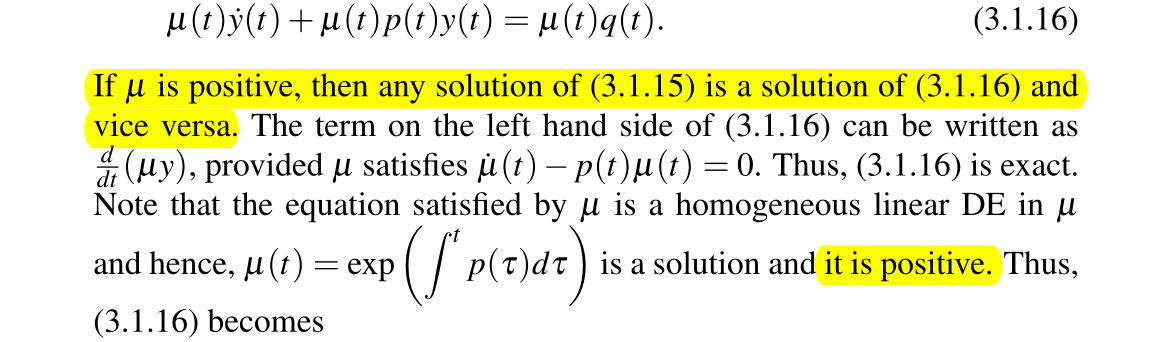
\includegraphics[scale=.30]{../assests/integrating_fac.png}}
    \caption{why $\mu$ has to be positive? Check this.}
    \label{fig1}
\end{figure}
Here $\mu(t)$ is called {\it integrating factor} associated with homogeneous part.

\subsection{Exact Differential equations}
\begin{defn}[Exact Differential equations]
    If the differential equation $ \dot{y} = f(t, y)$ can be written as $\frac{d}{dt}\phi(t,y(t)) = 0$ for a two variable function $\phi$ in a domain in the $t-y$ plane, then the differential equation is said to be an exact differential equation.
\end{defn}
\paragraph{\bf Necessary condition for DE to be exact}
Consider the differential form $Mdt + Ndy$, this can be written as general first order equation as
$$ M(t,y) + N(t,y) \dot{y} = 0$$
Above DE is exact {\it if and only if} there exists $\phi$ such that $\frac{d}{dt}\phi(t,y) = 0$. Therefore,
$$ \frac{\partial}{\partial t}\phi(t,y) + \frac{\partial}{\partial y}\phi(t,y)\dot{y} = M(t,y) + N(t,y) \dot{y} $$ and this implies 
$$ M = \frac{\partial \phi}{\partial t} \text{ and } N = \frac{\partial \phi}{\partial y}.$$
Assuming $\phi$ is double differentiable, we get 
$$ \frac{\partial M}{dy} = \frac{\partial N}{dt}$$
\begin{thm}
    Assume $M,N$ are defined on a rectangle $D = (a,b) \times (c,d)$ and $M,N \in C^1(D)$. Then, there exists a function $\phi$ defined in $D$, such that $M = \frac{\partial \phi}{\partial t}$ and $N = \frac{\partial \phi}{\partial y}$ if and only if $\frac{\partial M}{\partial y} = \frac{\partial N}{\partial t}$.
\end{thm}
\begin{proof}
    $(\implies)$ Assume there exists a function $\phi$ following the needed conditions given in theorem. The first relation $M = \frac{\partial \phi}{\partial t}$ suggests that $\phi(t, y) = \int M dt + h(y) $ for some $h$. Hence,
    $$ N = \frac{\partial \phi}{\partial t} = \int \frac{\partial M}{\partial y} dt + \frac{\partial h(y)}{\partial y} \implies \frac{\partial h}{\partial y} = N - \int \frac{\partial M}{\partial y} dt $$
    Since, LHS is a function of $y$ alone hence RHS should be a function of $y$ alone. Therefore,
    $$ \frac{\partial}{\partial t}\left(N - \int \frac{\partial M}{\partial y} dt\right) = 0 \implies \frac{\partial N}{\partial t} - \frac{\partial M}{\partial y} = 0$$
    $(\impliedby)$ Assume $M$ and $N$ satisfies $\frac{\pd M}{\pd y} = \frac{\pd N}{\pd t}$. Let a point $(t_0, y_0) \in D$. Define $\phi(t,y) = \int_{t_0}^{t} M(s,y) ds + h(y)$ where $h$ has to be determined. 
    \begin{align*}
        \frac{\pd \phi(t,y)}{\pd y} &= \int_{t_0}^{t} \frac{\pd M(s,y)}{\pd y} ds + \frac{\pd h(y)}{\pd y} \\
        &= \int_{t_0}^{t} \frac{\pd N(s, y)}{\pd t} ds + \frac{\pd h(y)}{\pd y}\\
        &= N(t, y) - N(t_0, y) + \frac{\pd h(y)}{\pd y}
    \end{align*}
    If we want $\frac{\pd \phi}{\pd y}$ to be equal to $N(t,y)$ then $\frac{\pd h(y)}{\pd y} = N(t_0,y) \implies h(y) = \int_{y_0}^{y} N(t_0, \xi) d\xi$. Therefore, 
    $$ \phi (t, y) = \int_{t_0}^{t} M(s, y) ds + \int_{y_0}^{y} N(t_0, \xi) d\xi$$ 
    $\phi$ is determined upto a constant. Hence on changing the point $(t_0, y_0)$ the constant term in $\phi$ will change. We may discard all the constant in expression of $\phi$.
\end{proof}
\begin{defn}[Alternate definition of Exact ODE]
    The DE, $M(t,y) + N(t, y)\dot{y} = 0$ is said to be exact if $\frac{\pd M}{\pd y} = \frac{\pd N}{\pd t}$.     
\end{defn}
\paragraph{\bf Solution of exact DEs} If a DE is exact then it can be written as $\frac{\pd \phi}{\pd t}(t,y) = 0$ and the solution of this DE can be written as $\phi = constant$.

\section{Second order linear equations} 
A second order linear differential equation is given by 
$$ Ly \equiv \ddot{y} + p(t)\dot{y} + q(t)y = r(t). $$
The operator $ Ly = L(t, y, \dot{y}, \ddot{y})$ is a multi-linear operator (linear in each of its variable). The IVP for second order linear ODE is given by
$$
\left.
\begin{array}{l}
    \ddot{y} + p(t)\dot{y} + q(t)y = r(t), t\in I \\
    y(t_0) = y_0, \dot{y}(t_0) = y_1    
\end{array}
\right\}
$$
\begin{thm}
    Let $p,q,r$ be continuous functions defined in a compact interval $I(t_0)$ and $y_0, y_1$ be any real numbers. Then, the IVP above has a unique solution $y$ defined in $I(t_0)$ satisfying $y(t_0) = y_0$ and $\dot{y}(t_0) = y_1$
\end{thm}
\begin{lem}
    Wronskian $W(z,w) \equiv 0$ if and only if $z$ and $w$ are dependent. Alternatively, $W \not\equiv 0$ if and only if $z$ and $w$ are independent. 
\end{lem}
\begin{proof}
    Let $t_0 \in I$ be a point in interval $I$ on which $z$ and $w$ are defined. Then the Wronskian is given by
    $$  W = \begin{vmatrix}
        z(t_0) & w(t_0) \\
        \dot{z}(t_0) & \dot{w}(t_0) 
    \end{vmatrix}
    $$
    This comes from the linear system (for $y_0$ and $y_1$ check next theorem)
    $$ \left\{
        \begin{array}{l}
            z(t_0)\alpha + w(t_0) \beta = y_0 \\
            \dot{z}(t_0) \alpha + \dot{w}(t_0) \beta = y_1 
        \end{array}
        \right.
    $$
    $(\impliedby)$ If $z = kw$ or $w = kz$ then the $W \equiv 0$.\\
    $(\implies)$ Assume that $W \equiv 0 \implies z\dot{w} - \dot{z}w = 0$
    \begin{align*}
        z\frac{dw}{dt} &= \frac{dz}{dt}w \\
        \int \frac{dw}{wdt} \times dt &= \int \frac{dz}{zdt} \times dt \\
        \ln w &= \ln z + c\\
        w &= e^{\ln z}e^c\\
        w &= ze^c
    \end{align*} 
    Therefore, $w$ and $z$ are dependent.
\end{proof}
\begin{thm}
    Let $z,w$ be two solutions of the linear homogeneous second order DE. Then, for any $\alpha, \beta \in \R$, the function $y = \alpha z + \beta w$ is also a solution.\\ Further, if $z$ and $w$ are two linearly independent solution of the homogeneous DE in an interval $I(t_0)$, then every solution $y$ can be written as $\alpha z + \beta w$.
\end{thm}
\begin{proof}
    First part of the theorem is trivial to verify. Let $y$ be a solution of the homogeneous DE. For some $t_0 \in I$, $y(t_0) = y_0 $ and $\dot{y}(t_0) = y_1$. We want to show that there exists $\alpha$ and $\beta$ such that $y(t) = \alpha z(t) + \beta w (t)$. Since $z$ and $w$ are independent, $W \not\equiv 0$ then there exists a unique solution to the linear system
    $$ \left\{
    \begin{array}{l}
        z(t_0)\alpha + w(t_0)\beta = y_0 \\
        \dot{z}(t_0) \alpha + \dot{w}(t_0) \beta = y_1
    \end{array}
    \right.
    $$
    Hence, there exists $\alpha $ and $\beta$. Here, $z$ and $w$ are basis elements for the solution space of second order linear homogeneous DE. Therefore, all the solution for this equation can be written in this form.
\end{proof}
\begin{thm}
    $\dim(S) = 2$ where $S$ is the solution space of second order linear homogeneous DE.
\end{thm}
\begin{proof}
    TODO
\end{proof}
\begin{rem}
    For $n$-th order linear homogeneous DE, the solution space is $n$-dimensional.
\end{rem}
\subsection{Non-homogeneous equations}
\begin{equation}\label{1}
    Ly := \ddot{y} + p(t)\dot{y} + q(t)y = r(t)
\end{equation}
\begin{thm}
    Assume that the functions $p$, $q$ and $r$ in (\ref{1}) are continuous. Let $S$ and $\tilde{S}$ be respectively, the solution set of homogeneous equation and non homogeneous equation. Then, $S$ is a linear space of dimension $2$ and $\tilde{S}$ is an affine space given by $\tilde{S} = S + y_p$ for any particular solution $y_p$ of (\ref{1}).
\end{thm}
\begin{proof}
    The assumption of continuity is needed for existence of solution. We have already proved in theorem $15$ that the dimension of $S$ is $2$. Since, any linear combination of solution is a solution and scalar times the solution is a solution, $S$ is linear.\\
    For some arbitrary $y \in \tilde{S}$ and let some $y_p$ be a particular solution for (\ref{1}). Since $Ly = r(t)$ and $Ly_p = r(t)$ implies that $L(y-y_p) = 0$ (due to linearity of operator $L$) then $y - y_p$ is a solution of homogeneous equation. Hence, by theorem $14$, $y - y_p = \alpha z + \beta w$ where $z$ and $w$ are two independent solutions of homogeneous equation. Also, $y$ is arbitrary
    \begin{align*}
        y &= \alpha z + \beta w + y_p\\
        \tilde{S} &= S + y_p        
    \end{align*}
\end{proof}
\paragraph{\bf Method of variation of parameters} This method can be used to find the particular solution, given the two independent solutions of corresponding homogeneous equation.\\
If $y_1(t)$ and $y_2(t)$ are the two independent solutions of homogeneous equation. We seek the solution to non homogeneous equation of the form 
$$ y(t) = c_1(t)y_1(t) + c_2(t)y_2(t) $$
where $c_1(t)$ and $c_2(t)$ are the functions to be determined. Compute $Ly(t) = r(t)$, and then assume $\dot{c_1}y_1 + \dot{c_2}y_2 = 0$ to be one equation. Another equation can be found by substituting above assumption in $Ly(t) = r(t)$. Then by solving this system, we can find $c_1(t)$ and $c_2(t)$ and $y_p(t) = y(t)$.




\section{Doubts}
\paragraph{\bf Ques 1} In linear equations with constant coefficient, how is $\dot{y} \propto y$?



\end{document}